\documentclass[tikz]{standalone}
\usepackage{pgfplots}
\pgfplotsset{width=7cm, compat=1.18}
\begin{document}
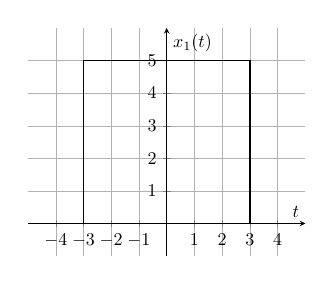
\begin{tikzpicture}[scale=0.65]
\begin{axis}[
	axis y line=center,
	axis x line=middle,
	xmin=-5,	xmax=5,
	ymin=-1,	ymax=6,
	xlabel={$t$},
	ylabel=$x_1(t)$,
	xtick={-4,-3,-2,-1,0,1,2,3,4},
	ytick={0,1,2,3,4,5},
	grid=both,
	grid style={line width=.1pt, draw=gray!40},
	major grid style={line width=.2pt,draw=gray!60},
	]
	\addplot[line width=.8pt] coordinates {(-3,0) (-3,5) (3,5) (3,0)};
\end{axis}	
\end{tikzpicture}
\end{document}
